\chapter{Implementacija i korisničko sučelje}
		
		
		\section{Korištene tehnologije i alati}
		
		
			
			 {Za međusobnu komunikaciju unutar tima korišten je Discord u kojem su članovi tima bili podijeljeni u nekoliko kanala kako bi se organizirali različiti dijelovi projekta. Također za svojevrsnu komunikaciju upotrebljavan je i GitHub što je jedna od najpoznatijih platformi koja omogućuje programerima da imaju repozitorije u kojima zatim mogu stvarati, pohranjivati i upravljati svojim kodovima i projektima. Također moguće je pratiti svaku promjenu. Prilikom izrade projekta GitHub je služio kako bi bila olakšana međusobna komunikacija te kako bi na jednom mjestu bilo dostupno sve što se radi na projektu u svakom trenutku.}
			 
			 {Za izradu dokumentacije korišten je sustav za uređivanje teksta LaTex. Ovaj markup jezik se najčešće koristi za izradu znanstvene i tehničke publikacije. Njegove prednosti su lakoća formatiranja velikih datoteka što olakšava i skraćuje vrijeme koje bi se potrošilo na uređivanje samog dokumenta. Prilikom izrade UML dijagrama korišten je Astah UML alat za modeliranje UML dijagrama. Poznat je po tome što je vrlo jednostavan za učenje i korištenje. Također brži je od Excela i drugih alata za crtanje. Astah je primijenjen prilikom izrade dijagrama obrazaca uporabe, sekvencijskih dijagrama, dijagrama baze podataka,  dijagrama razreda, stanja, aktivnosti, komponenti te dijagram razmještaja.Za izradu frontenda korišten je Angular te jezik Typescript dok su za backend korišteni .NET Framework i jezik C}
			 
			 
			 
			 {Angular je platforma tj. okvir (eng. Framework) koji služi za razvijanje web aplikacija pomoću TypeScript-a i HTML-a. Kako bi se mogao koristiti Angular potrebno je prethodno instalirati NPM te Node.js. Prednost Angular-a je kod koji je lako čitljiv te koji se može ponovno iskoristiti, također dobra je tehnologija za rad u timu s obzirom da omogućuje usporedan samostalan rad. Radni okvir .NET Framework namijenjen je za izgradnju i izvođenje aplikacija. Korišteni su i Visual Studio Code i Visual Studio. To su integrirana razvojna okruženja (eng. IDE). Koriste se kao platforma za uređivanje izvornog koda te platforma za  pokretanje koja se može koristiti za uređivanje, debugiranje, izgradnju koda i samo objavljivanje aplikacije.}
			 
			 
			 {PGAdmin je korisničko grafičko sučelje iskorišteno za interakciju sa Postgres-om prilikom izrade baze podataka dok je EntityFramework korišten kao poveznica baze podataka i backend-a. Za dohvat početne informacije o parkirališnim mjestima upotrebljeno je aplikacijsko programsko sučelje Overpass, a za mapu je iskorišten Open Street Map. Također korišten je Nominatim koji služi za pretvaranje koordinata u adresu te OSRM Demo API koji koristi algoritme usmjeravanja za izračun i pronalazak najkraćeg puta do odredišta.}
			
			\begin{enumerate}
				
				
				\item   \url{https://discord.com/}
				
				\item   \url{https://github.com/}
				
				\item   \url{https://www.latex-project.org/}
				
				\item  \url{https://astah.net/products/astah-uml/}
				
				\item   \url{https://angular.io/}
				
				\item   \url{https://dotnet.microsoft.com/en-us/learn/dotnet/what-is-dotnet-framework}
				
				\item   \url{https://visualstudio.microsoft.com/}
				
				\item   \url{https://www.pgadmin.org/}
				
				\item   \url{https://learn.microsoft.com/en-us/aspnet/entity-framework}
				
				\item   \url{https://hrbrmstr.github.io/overpass/}
				
				\item   \url{https://www.openstreetmap.org/#map=7/44.523/16.460}
				
				\item   \url{https://nominatim.openstreetmap.org/ui/search.html}
				
				\item   \url{https://project-osrm.org/docs/v5.5.1/api/#introduction}
				
				
			\end{enumerate}
			
			\eject 
		
	
		\section{Ispitivanje programskog rješenja}
			
			
			
			 {Opisujemo provedbu ispitivanja implementiranih funkcionalnosti na razini komponenti i na razini cijelog sustava s prikazom odabranih ispitnih slučajeva.}
	
			
			\subsection{Ispitivanje komponenti}
			
			\textbf{DistanceFunctionTest}
			
			{Pri stvaranju instantne rezervacije traži se parkirno mjesto koje je najbliže traženoj destinaciji. Pri tome odlučili smo koristiti Haversinovu formulu. Za ovaj test odabrali smo pouzdan primjer za koji znamo točan odgovor te testirali vraća li funkcija ispravnu vrijednost:}
			
			\begin{figure}[h]
				\centering
				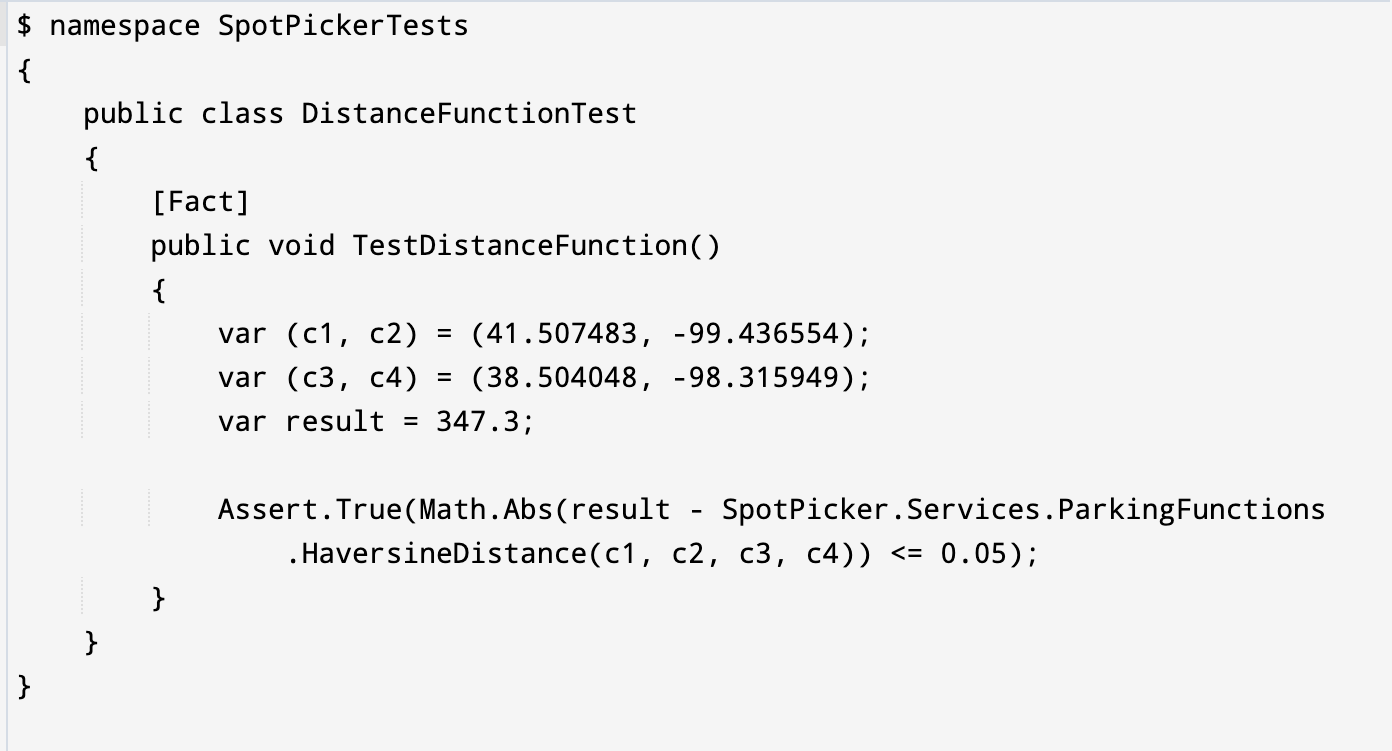
\includegraphics[width=\textwidth,keepaspectratio]{slike/kod1.png}
				\caption{DistanceFunctionTest}
				\label{fig:kod1}
			\end{figure}
			
			
			\textbf{IBanFunctionTest}
			
			{Pri mijenjanju IBAN-a od strane admina ili registraciji provjerava se validnost unesenog IBAN-a. Zato testiramo funkciju koja to provjerava pomoću ispravnog i neispravnog IBAN-a:}
			
			
		
			\begin{figure}[hbt!]
				\centering
				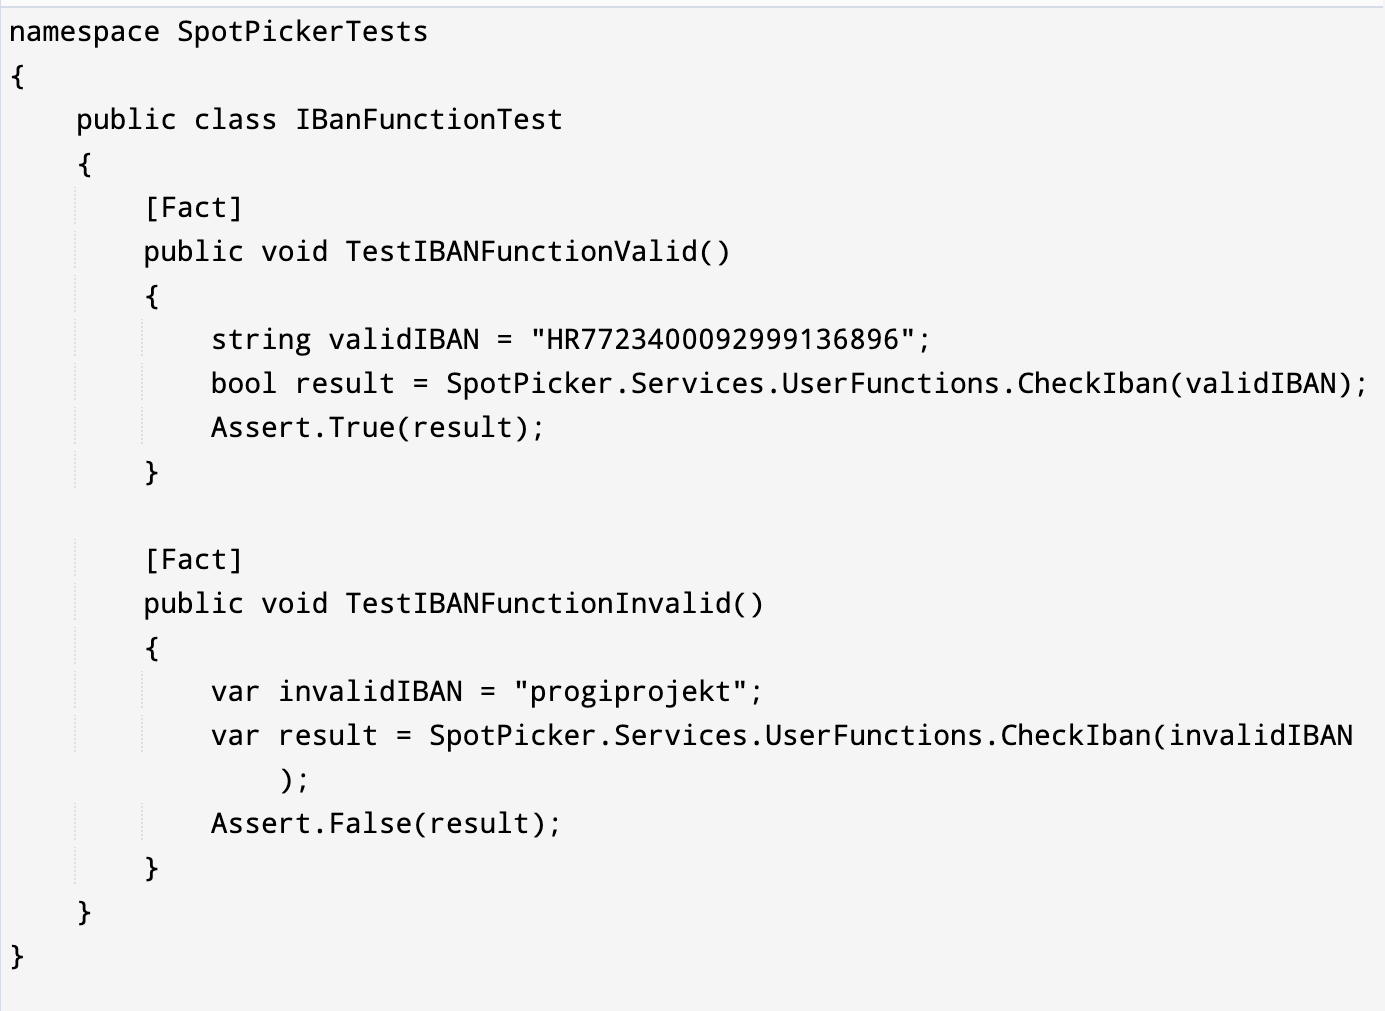
\includegraphics[width=0.7\linewidth]{slike/kod2.png}
				\caption{IBanFunctionTest}
				\label{fig:kod2}
			\end{figure}
			
			
			\textbf{PasswordRegexTest}
			
			{Pri registraciji unosi se lozinka, minimalna duljina je 8 znakova, uključujući minimalno jednu znamenku, zato testiramo tu funkciju s nekoliko primjera:}
			
			
			
			
			\begin{figure}[hbt!]
				\centering
				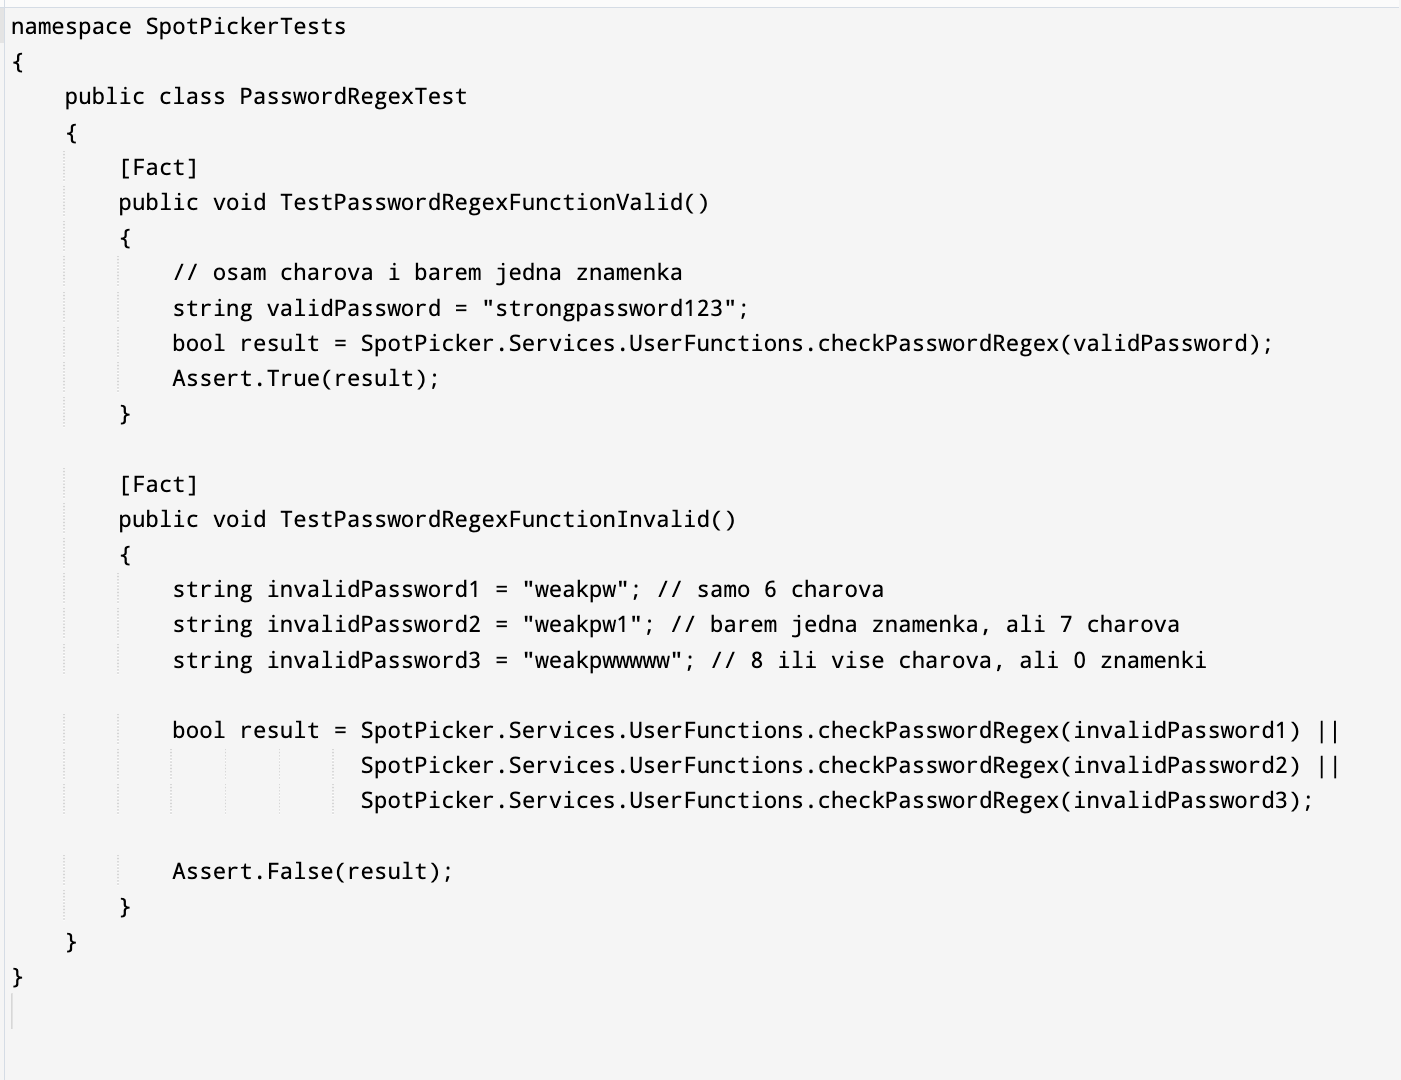
\includegraphics[width=0.7\linewidth]{slike/kod3.png}
				\caption{PasswordRegexTest}
				\label{fig:kod3}
			\end{figure}
			
			
			
		
			
			
			
			
			\subsection{Ispitivanje sustava}
			
			 \textbf{LoginTest}
			 
			 {Ovo je sistem test koji testira funkcionira li login (ulogira se u adminov profil):}
			 
			
			 
			
			 
			 \begin{figure}[hbt!]
			 	\centering
			 	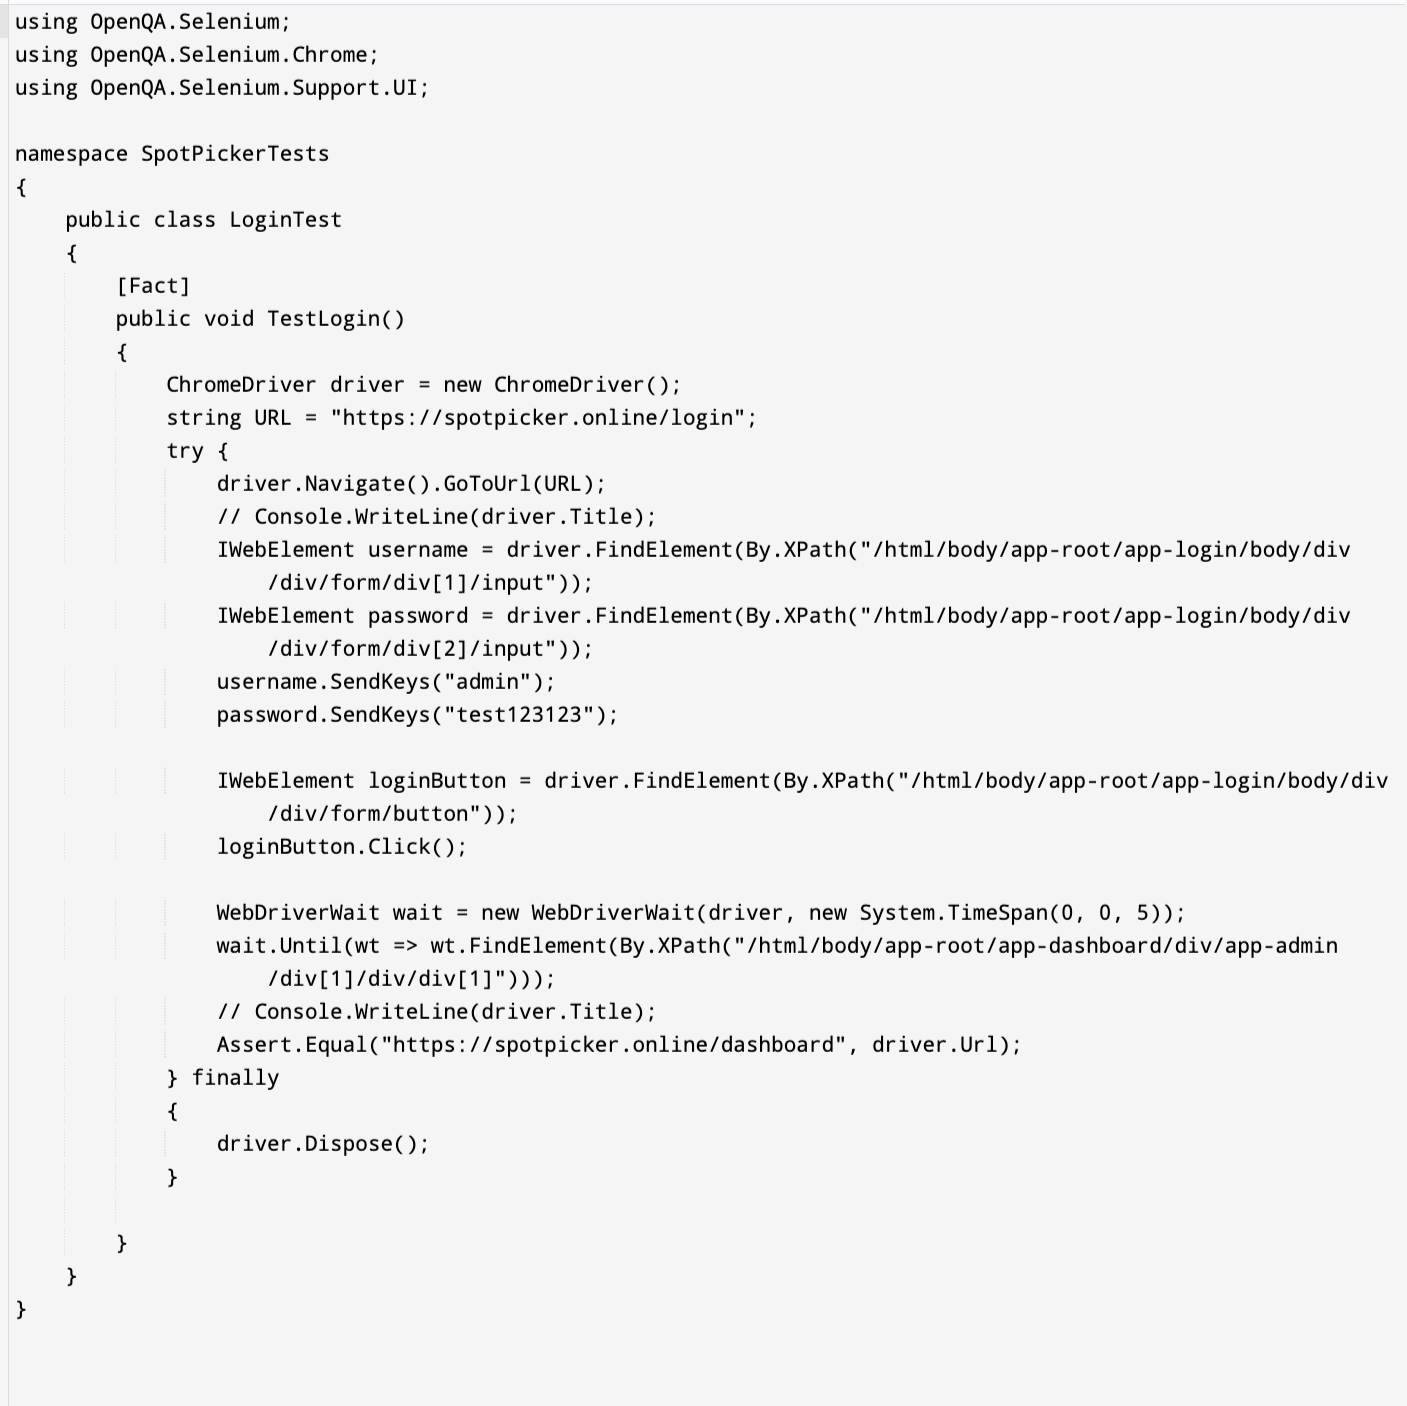
\includegraphics[width=0.7\linewidth]{slike/kod4.png}
			 	\caption{LoginTest}
			 	\label{fig:kod4}
			 \end{figure}
			 
			 
			 \textbf{AdminChangeTest}
			 
			 {Još jedan sistem test, ovaj provjerava funkcionira li promjena nečije uloge od strane admina:}
			 
			 
			 
			 \begin{figure}[hbt!]
			 	\centering
			 	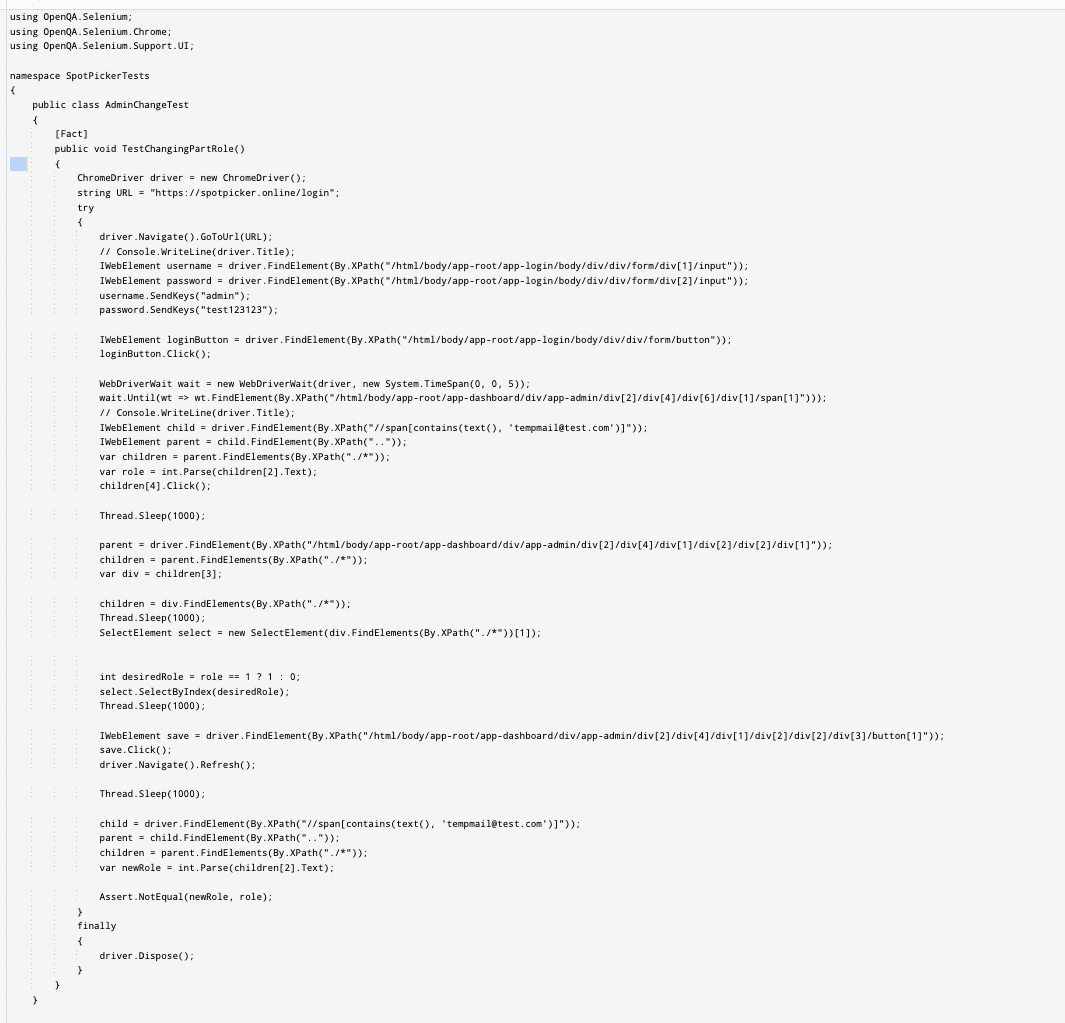
\includegraphics[width=0.7\linewidth]{slike/kod5.png}
			 	\caption{AdminChangeTest}
			 	\label{fig:kod5}
			 \end{figure}
			 
			 
			 
			 
			 {Za pokretanje testova koristili smo xUnit testing framework, ovo je rezultat:}
			 
			 
			 
			 
			 \begin{figure}[hbt!]
			 	\centering
			 	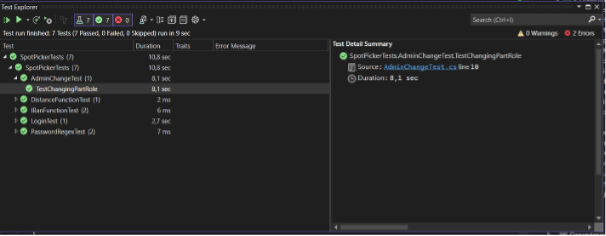
\includegraphics[width=0.7\linewidth]{slike/slikica6.png}
			 	\caption{xUnit testing framework}
			 	\label{fig:slikica6}
			 \end{figure}
			 
			 
			
			\eject 
		
		
		\section{Dijagram razmještaja}
			
			
			
			 {Kako bi se bolje razumjela arhitektura sustava koristi se dijagram razmještaja. On prikazuje arhitekturu programskog sustava tako što pokazuje razmještaj programske potpore i samu topologiju sklopovlja. Svrha dijagrama razmještaja je pružanje pomoći prilikom donošenja raznih odluka u vezi sustava. Poslužiteljsko računalo može obavljati veći broj radnji u isto vrijeme te ga u istom trenutku može koristiti više korisnika. Web poslužitelj te poslužitelj baze podataka nalaze se na poslužiteljskom računalu, a korisnici koriste web poslužitelj za pristup web aplikaciji. Korištena je klijent-poslužitelj arhitektura. Prednosti ove arhitekture je što više klijenata istovremeno može pristupiti poslužitelju te mogu pristupiti funkcionalnostima poslužitelja sa udaljenosti. Komunikacija između računala korisnika, administratora i voditelja parkinga je realizirana putem HTTP veze.}
			 
			 \begin{figure}[hbt!]
			 	\centering
			 	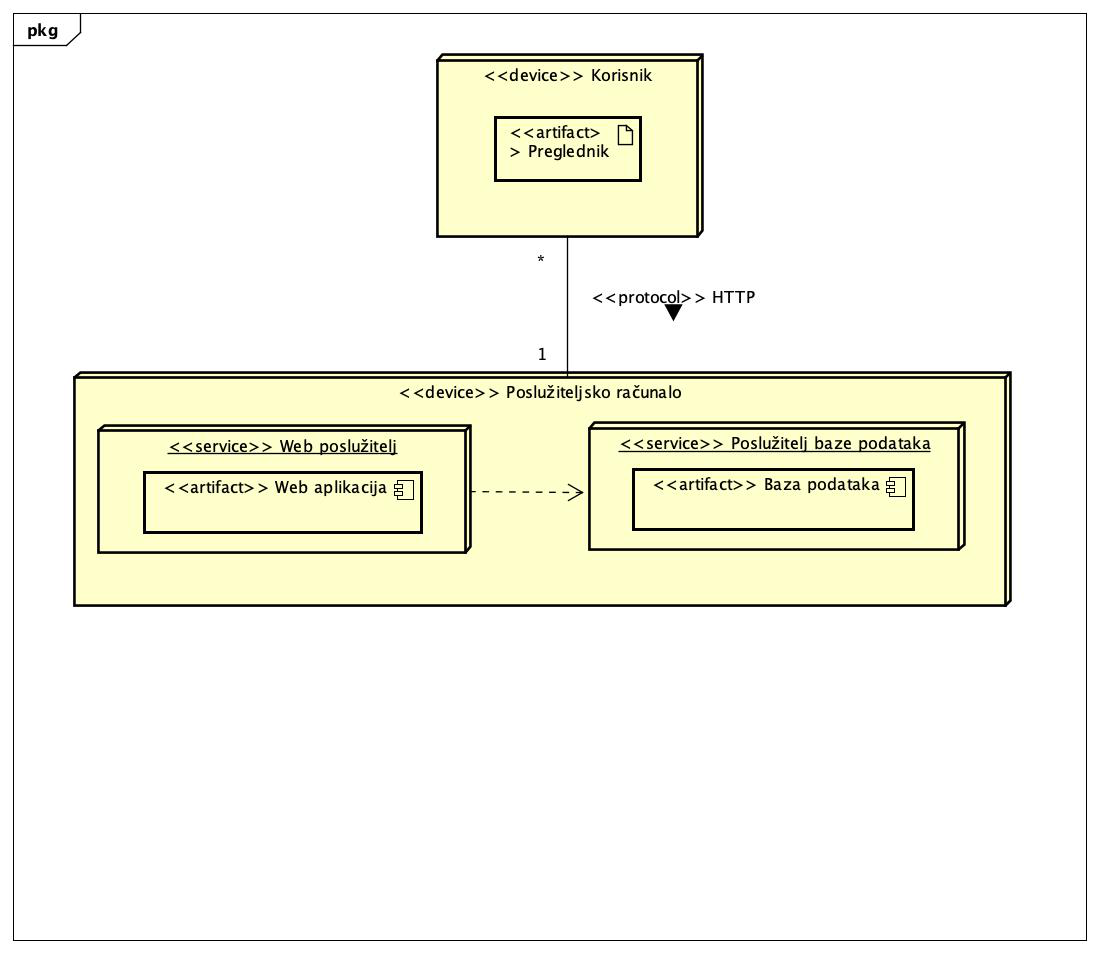
\includegraphics[width=0.7\linewidth]{slike/DijagramRazmjestaja.png}
			 	\caption{Dijagram razmještaja}
			 	\label{fig:DijagramRazmjestaja}
			 \end{figure}
			
			\eject 
		
		\section{Upute za puštanje u pogon}
		
			
		
			 {Postoji server odnosno računalo koje je smješteno u Nizozemskoj i na njemu je instaliran Nginx server koji poslužuje našu aplikaciju. Na tom remote računalu se nalazi frontend, backend i baza podataka. Baza podataka je PostgreSQL i ona je otvorena za konekcije svim IP adresama, potrebna je samo lozinka te se mi spojimo sa svojeg računala na tu bazu koja je u Nizozemskoj i onda ažuriramo nove podatke koje postavljamo. Na taj način bazu podataka ažuriramo i postavljamo, a frontend i backend prvo izgradimo i onda te datoteke pomoću FileZilla, software koji nam olakšava povezivanje sa serverom, pomoću SFTP protokola prebacujemo podatke na remote računalo odnosno naš server. }
			 
			 
			 \begin{figure}[hbt!]
			 	\centering
			 	\includegraphics[width=0.7\linewidth]{slike/datotečnisustav.png}
			 	\caption{prikaz povezivanja u datotečni sustav remote računala}
			 	\label{fig:datotečnisustav}
			 \end{figure}
			 
			 
			 
			 
			 
			 \begin{figure}[h]
			 	\centering
			 	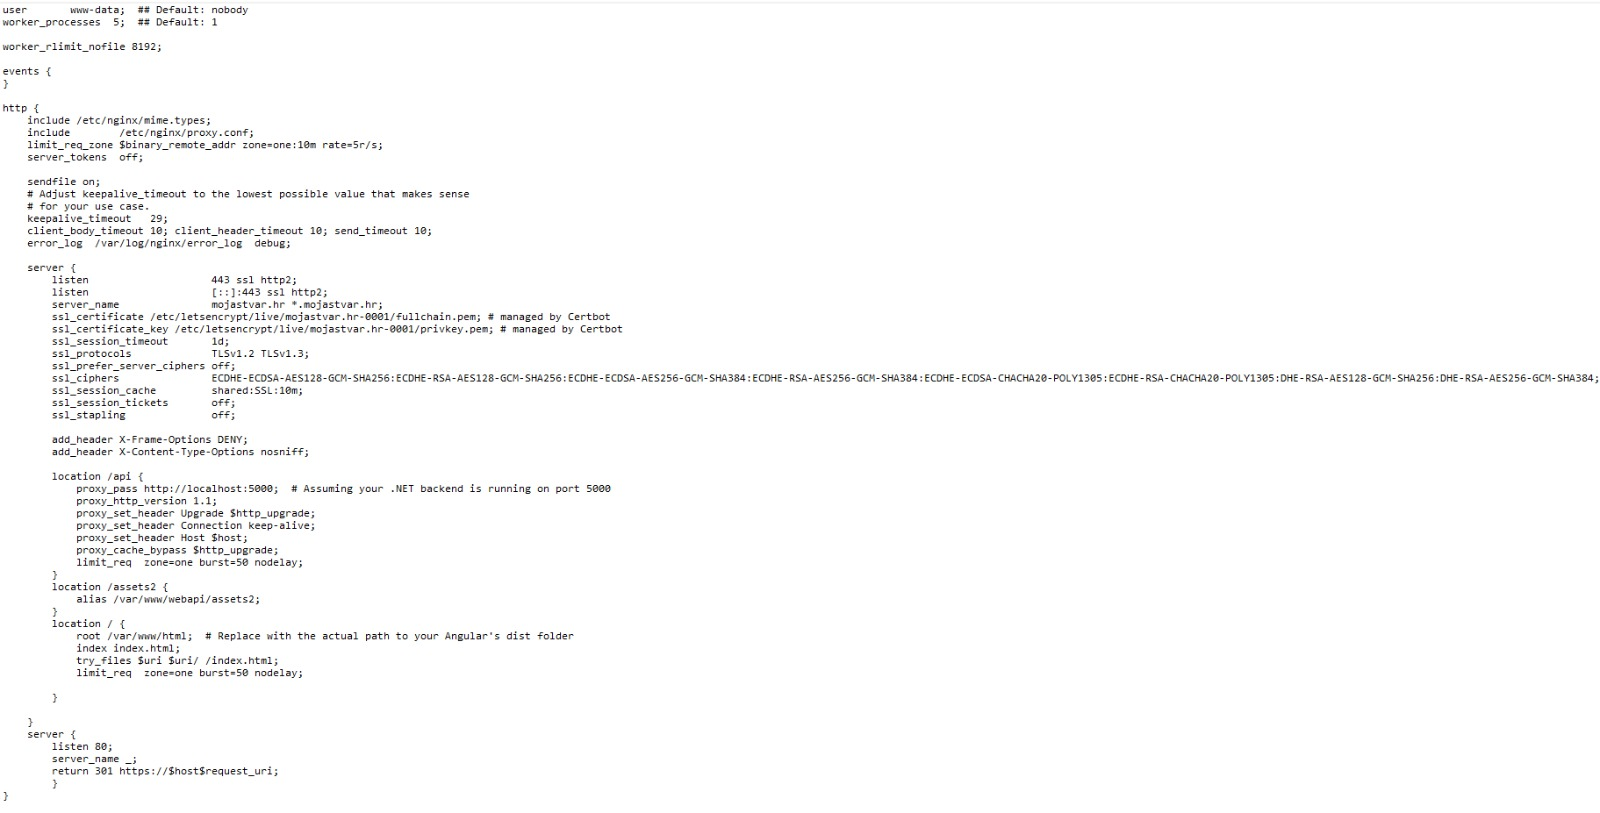
\includegraphics[width=\textwidth,keepaspectratio]{slike/konfiguracijaservera.png}
			 	\caption{prikaz konfiguracije servera}
			 	\label{fig:konfiguracijaservera}
			 \end{figure}
			 
			 
			 
			 \begin{figure}[hbt!]
			 	\centering
			 	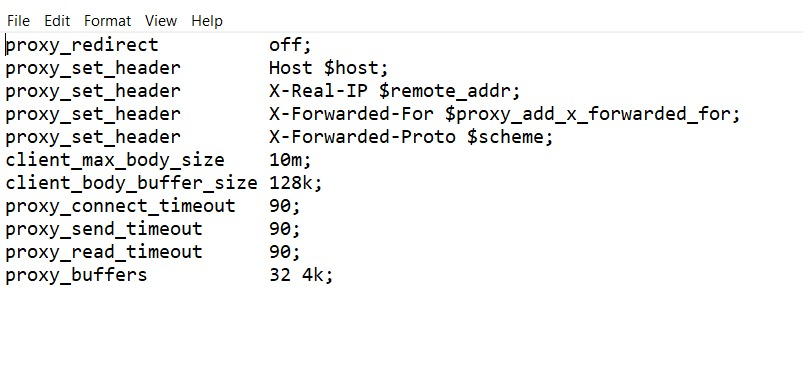
\includegraphics[width=0.7\linewidth]{slike/konfiguracijaproxyja.png}
			 	\caption{prikaz konfiguracije proxyja}
			 	\label{fig:konfiguracijaproxyja}
			 \end{figure}
			 
			 
			 
			 \begin{figure}[hbt!]
			 	\centering
			 	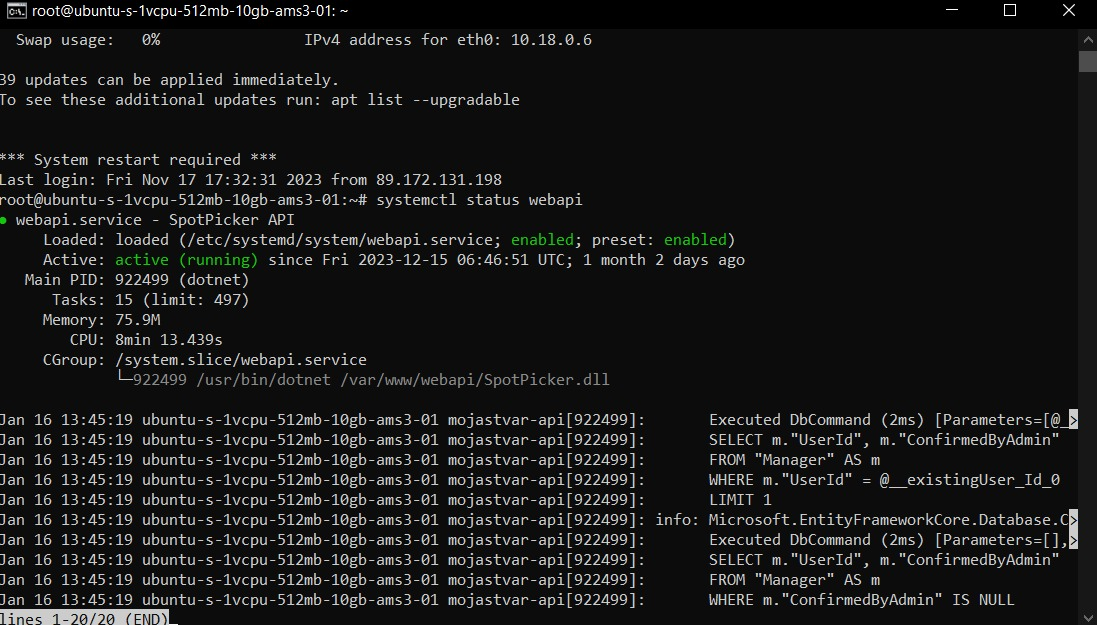
\includegraphics[width=0.7\linewidth]{slike/povezivanjekonzole.png}
			 	\caption{prikaz povezivanja preko konzole na Ubuntu server}
			 	\label{fig:povezivanjekonzole}
			 \end{figure}
			 
			
			
			 
			
			
			\eject 